\documentclass{beamer}

\usepackage[utf8]{inputenc}
\usepackage[french]{babel}

\usetheme{Warsaw}

\title[Service Routière]{Implémentation de Service de Collecte et de Stockage des Données sur une plateforme de services Routières}
%\subtitle{Mémoire de projet de fin d'études}
\author{Moez Bouhlel \and Rihab Majdoub}
\author[Moez B. \and Rihab M.]{\textbf {Moez Bouhlel \and Rihab Majdoub\\ \footnotesize Sour la direction de: Dr. Mohammed Amri}}
\institute{Faculté des Sciences de Sfax}
%\logo{
\includegraphics[width=4cm]{figures/logo-djagora.png}}
%\logo{
\includegraphics[width=2cm]{figures/fss-old.eps}}
\titlegraphic{
\includegraphics[width=2cm]{figures/fss-old.eps}}
\date{05/06/2017}
\begin{document}
{
    \makeatletter
        \setbeamertemplate{headline}[default] % not mandatory, but I though it was better to set it blank
            \def\beamer@entrycode{\vspace*{-\headheight}} % here is the part we are interested in :)
            \makeatother
\frame{\titlepage}
}

\begin{frame}
\frametitle{Plan de la présentation}
\tableofcontents[hideallsubsections]
\end{frame}
\AtBeginSection[]
{
  \begin{frame}
    \frametitle{Plan de la présentation}
    \tableofcontents[currentsection,hideothersubsections]
  \end{frame}
}

\section{Introduction Générale}
\begin{frame}
\frametitle{Organisme d'accueil}
\framesubtitle{Djagora Academy}
\begin{figure}
    
\includegraphics[width=.7\textwidth]{figures/logo-djagora.png}
\end{figure}
\end{frame}

\begin{frame}
    \frametitle{Présentation du projet}
    \framesubtitle{Équipe City Watch}
\begin{figure}
    
\includegraphics[width=.6\textwidth]{figures/logo-citywatch.jpg}
\end{figure}
\end{frame}

\begin{frame}
    \frametitle{Problématique}
    
\includegraphics[width=.6\textwidth]{figures/datamanagement-issues.jpg}
    
\includegraphics[width=.32\textwidth]{figures/question.png}
\end{frame}

\begin{frame}
    \frametitle{Présentation du projet}
    \framesubtitle{Objectif}
    \begin{columns}
        \begin{column}{0.5\textwidth}
            \begin{figure}
                
\includegraphics[width=1\textwidth]{figures/logo-citywatch.jpg}
            \end{figure}
        \end{column}
        \begin{column}{0.5\textwidth}
            \begin{itemize}
                \item<1-> Collecte des données
                \item<2-> Analyse des données
                \item<3-> Valorisation des données
            \end{itemize}
        \end{column}
    \end{columns}
\end{frame}

\begin{frame}
    \frametitle{Présentation du projet}
    \framesubtitle{Architecture}
    \begin{figure}
        \centering
    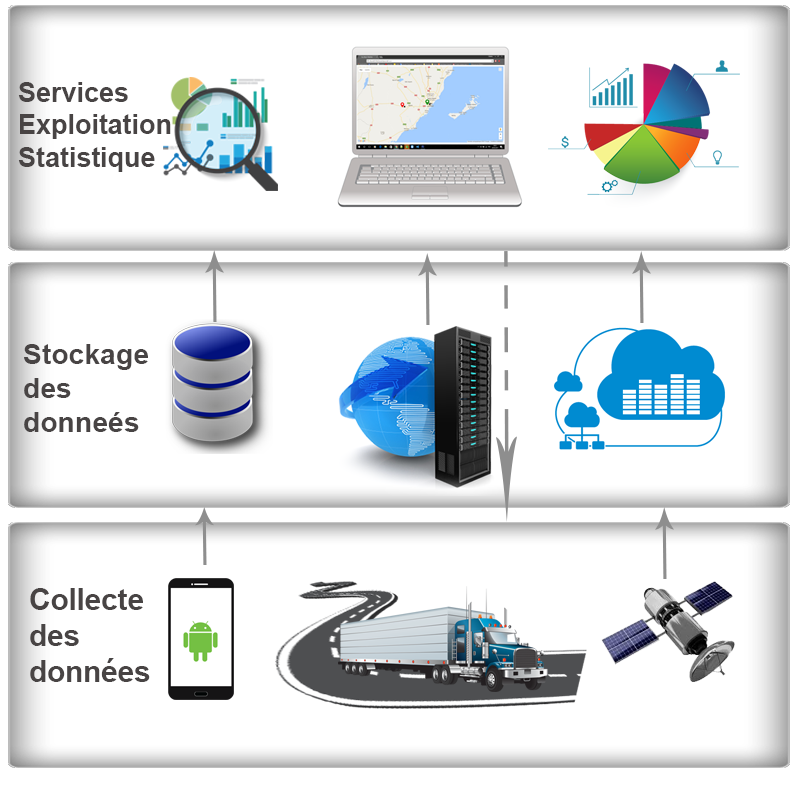
\includegraphics[width=.63\textwidth]{figures/citywatch-modules.png}
\end{figure}
\end{frame}

\begin{frame}
    \frametitle{Gestion du projet}
    \framesubtitle{Scrum}
    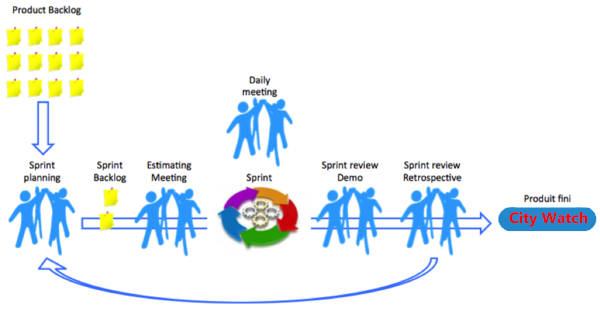
\includegraphics{figures/scrum-model.png}
\end{frame}

\section{Réalisation}
\subsection{Itération 1}
\subsection{Itération 2}
\subsection{Itération 3}
\begin{frame}
    \frametitle{}
\end{frame}

\begin{frame}
    \frametitle{}
\end{frame}

\section{Démonstration}
\begin{frame}
    \begin{center}
        \textbf{\Huge Démo}
    \end{center}
\end{frame}

\section{Conclusion}
\begin{frame}
    \frametitle{Conclusion}
\end{frame}

\section{Perspectives}
\begin{frame}
    \frametitle{Perspectives}
\end{frame}

\end{document}
